\documentclass[11pt,a4paper]{article}

% ---- Packages ----

 % Section titles
\usepackage[T1]{fontenc}
\usepackage{biolinum}

% Default sans-serif font for body text
\usepackage[sfdefault]{classico}
\usepackage[scale=0.9]{FiraMono}

% Default monospace font
\renewcommand{\ttdefault}{FiraMono-TLF}

\usepackage[margin=1cm]{geometry}
\usepackage{graphicx}        % photo
\usepackage{xcolor}
\usepackage{enumitem}
\usepackage{titlesec}
\usepackage{microtype}   % provides \lsstyle for letterspacing
\usepackage{hyperref}
\usepackage{fontawesome5}     % icons for phone/mail/github
\usepackage{tabularx}
\usepackage{tikz}             % rounded-corner image clip
\usepackage{needspace}        % keep blocks together across page breaks

% ---- Colors ----
% #2C3E50
% #4d5d5f
% #525f4d
% #43503f
\definecolor{accent}{HTML}{43503f}

% #d1d8d8
% #7f8c8d

% #d1d8d2
% #7f8d87
\definecolor{gray}{HTML}{7f8d87}
\definecolor{lightgray}{HTML}{d1d8d2}

% ---- Hyperlinks ----
\hypersetup{
  colorlinks=true,
  urlcolor=accent,
  linkcolor=accent
}

% ---- Section style ----
\titleformat{\section}
  {\large\bfseries\fontfamily{LinuxBiolinumT-TLF}\selectfont\color{accent}}
  {}{0em}{}[\titlerule]
\titlespacing{\section}{0pt}{12pt}{6pt}

% ---- Remove page numbers ----
\pagestyle{empty}

% ---- Helper for experience / education entries ----
% \entry{Title}{Subtitle}{Date}
\newcommand{\entry}[3]{%
  \noindent\textbf{#1} 
  \textcolor{gray}{\textit{#2}}
  \hfill \textcolor{gray}{#3}\par\vspace{2pt}
}

\newcommand{\caret}{\ \ {\color{lightgray}\faCaretRight}\ \ }

\begin{document}

% =====================================================
% HEADER
% =====================================================
\noindent
\begin{minipage}[c]{0.2\textwidth}
  \tikz\node[inner sep=0pt, rounded corners=2pt, clip]
    {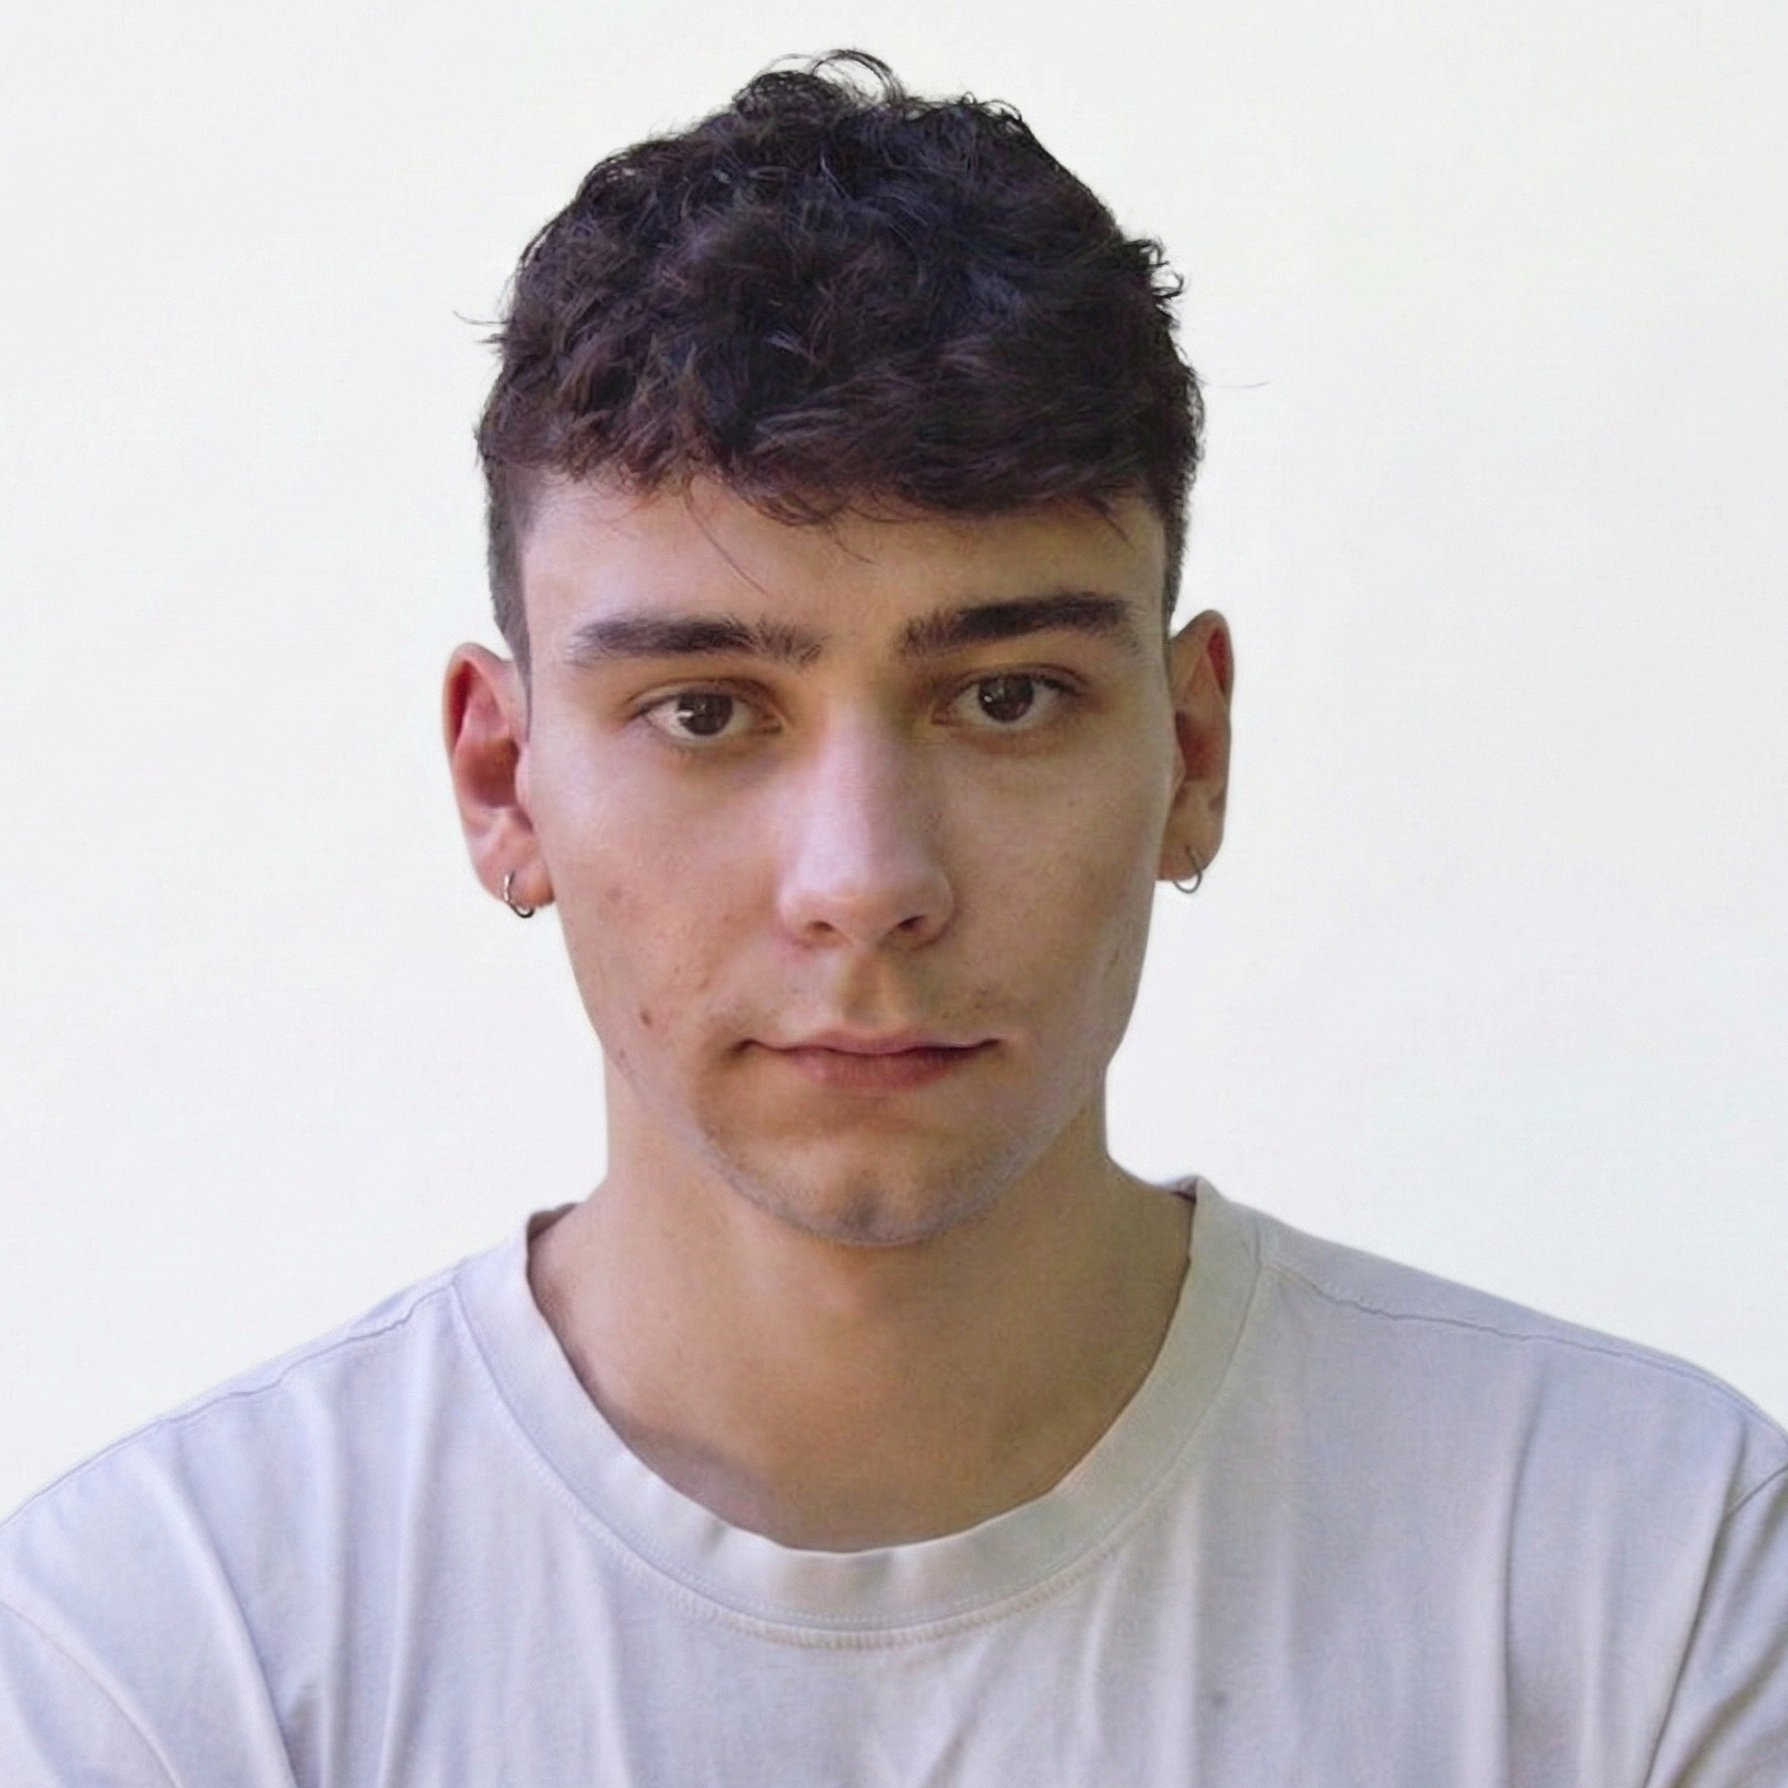
\includegraphics[width=3cm,height=3cm,keepaspectratio]{media/me.png}};
\end{minipage}\hfill
\begin{minipage}[c]{0.35\textwidth}
  {\Large Lorenzo Celli}\\[10pt]
  \begin{tabularx}{\textwidth}{@{}c@{\hspace{10pt}}X@{}}
    {\color{gray}\faEnvelope} & \small{\href{mailto:lorenzo.celli00@gmail.com}{lorenzo.celli00@gmail.com}} \\
    {\color{gray}\faGithub} & \small{\href{https://github.com/lorenzocelli}{github.com/lorenzocelli}} \\
    {\color{gray}\faLink} & \small{\href{http://lorenzocelli.me}{lorenzocelli.me}}
  \end{tabularx}
\end{minipage}
\begin{minipage}[c]{0.4\textwidth}
  \vspace{18pt}
  \begin{tabularx}{\textwidth}{@{}c@{\hspace{8pt}}X@{}}
    {\color{gray}\faMapMarker*} & \small{Zürich}\\
    {\color{gray}\faGlobeAfrica} & \small{Italian, B permit}
  \end{tabularx}
\end{minipage}
\vspace{10pt}

% =====================================================
% SUMMARY
% =====================================================
\noindent
Computer scientist with a strong interest in computer graphics, computational geometry, computer vision, and machine learning. Originally from Bologna, now based in Zürich where I am pursuing my Master's degree.

% =====================================================
% PROFESSIONAL EXPERIENCE
% =====================================================
\section{Professional Experience}
\entry{Research Assistant}{ETH (Safespace Research), Zürich}{2025\caret Present}
\begin{itemize}[leftmargin=*,nosep]
  \item Implemented a Graph-RAG system for enhanced LLM generation targeted at mental health support.
  \item Developed the frontend of a mobile application for iOS and Android with React Native, Xcode, Android Studio. Developed a REST API with Django and Django REST Framework. Deployed with Docker on Azure.
\end{itemize}
\vspace{6pt}

\entry{CAD Software Engineer}{devDept, Bologna}{2020\caret 2024}
\begin{itemize}[leftmargin=*,nosep]
  \item Worked on a 3D CAD framework library in C\#, focusing on geometric modeling and performance. Meshing of NURBS surfaces and B-Reps (\href{https://www.youtube.com/watch?v=tZCLl7WwqoM}{video}), mesh editing (\href{https://www.youtube.com/watch?v=23w_LPZiCwo}{video}), CNC simulation and toolpath generation.
  \item Developed a debugging tool for 3D shapes called \href{https://devdept.zendesk.com/hc/en-us/articles/19007089043996-Blink-Debugging-Tool}{Blink}.
\end{itemize}
\vspace{6pt}

\entry{ECMWF Summer of Weather Code}{ECMWF, Reading}{2019}
\begin{itemize}[leftmargin=*,nosep]
  \item Extended the Blender add-on BVTK for processing and visualization of meteorological data. Animations were displayed at the 2019 AGU (American Geophysical Union) meeting. 
\end{itemize}
\vspace{6pt}

\entry{Python Developer for Scientific Computing}{CINECA, Bologna}{2018\caret 2019}
\begin{itemize}[leftmargin=*,nosep]
  \item Developed a Blender add-on (BVTK) integrating scientific visualization via the VTK library.
  \item Presented at the Blender Conference in 2018.
\end{itemize}

% =====================================================
% EDUCATION
% =====================================================
\section{Education}

\entry{MSc Computer Science}{ETH Zürich}{2024\caret Present}
\begin{itemize}[leftmargin=*,nosep]
  \item Major in Visual and Interactive Computing, minor in Machine Learning.
\end{itemize}
\vspace{6pt}

\entry{Overseas Exchange Program}{University of Technology Sydney}{2022}
\vspace{6pt}

\entry{BSc Computer Engineering}{University of Bologna}{2019\caret 2022}
\begin{itemize}[leftmargin=*,nosep]
  \item Thesis: \textit{Tessellation of boundary represented CAD models (B-Rep)}.
  \item Graduated with honors and won two scholarships for academic merit in 2019 and 2020.
\end{itemize}

% =====================================================
% PROJECTS
% =====================================================
\Needspace*{8\baselineskip}
\section{Selected Projects}
\entry{Semester Project}{Computational Robotics Lab, ETH Zürich}{2026}
\begin{itemize}[leftmargin=*,nosep]
  \item Developed Vorotile, a Voronoi-based generator of tileable patterns, supporting characterization of the mechanical properties of the resulting microstructures via homogenization analysis. Implemented in Python with JAX, NumPy, and Matplotlib. Web demo with vanilla WebGL.
\end{itemize}
\vspace{6pt}

\entry{Implicit SPH}{Physically Based Simulations for Computer Graphics, Course Project}{2025}
\begin{itemize}[leftmargin=*,nosep]
  \item Implemented in \texttt{C++} an implicit Smoothed Particle Hydrodynamics (SPH) solver for elastic solids simulation, based on the paper ``An Implicit SPH Formulation for Incompressible Linearly Elastic Solids'' by Peer et al. (repository: \href{https://github.com/lorenzocelli/implicit-sph}{github.com/lorenzocelli/implicit-sph}).
\end{itemize}

% =====================================================
% TECHNICAL SKILLS
% =====================================================
\section{Technical Skills}
\begin{tabularx}{\textwidth}{@{}lX@{}}
  \textbf{Programming Languages} & Python, \texttt{C}, \texttt{C++}, \texttt{C\#}, Java, Rust, Julia \\
  \textbf{Web Frameworks} & React, React Native, Next.js, Tailwind, Django, Django REST Framework \\
  \textbf{Tools} & Git, Docker, Linux, LaTeX
\end{tabularx}

% =====================================================
% LANGUAGE SKILLS
% =====================================================
\section{Language Skills}
\begin{tabularx}{\textwidth}{@{}ll@{\hspace{2em}}lX@{}}
  \textbf{Italian} & Native &
  \textbf{English} & Fluent (C1)
\end{tabularx}

\end{document}
